\section{Experiments}\label{sec:experiments}



The proposed multi-user preference learning model is evaluated in a series of experiments with simulated data.
We generate a total of $I=15$ synthetic items with features given by 2-dimensional vectors,
where the $i$-th item satisfies
$\x_i=(x_{i1},x_{i2})$ with $x_{i1},x_{i2} \sim U[-5, 5]$. The preferences of each user are given
by a linear combination of $D=5$ latent functions $h_1,\ldots,h_5$. These functions are sampled from a Gaussian process
with zero mean and preference covariance function generated by a squared exponential kernel with unit length-scale.
The preferences for the $u$-th user are obtained according to 
$g_u(\x, \x') = \text{sign}\{ \sum_{d=1}^5 w_{ud} h_d(\x, \x') + \epsilon_{\x,\x'} \}$,
where $w_{u1},\ldots,w_{u5}$ and $\epsilon_{\x, \x'}$ are sampled from a standard Gaussian distribution.
All the possible pairwise preferences are evaluated for a total of $U = 200$ users. 
For each of these users, the available preference data are randomly split into training, pool and test sets with 10, 20 and 15 elements, respectively.
In total, we have 200 training, pool and test sets, one per each different user.
The multi-task model is fitted using the data available in the 200 training sets and its performance is
evaluated on the corresponding test sets. After this, the most informative data point is identified in each of the 200 pool sets.
The resulting 200 data points are then moved into the corresponding training sets and the whole process repeats
again until 10 of these active additions to the training sets have been completed.
The spliting of the data into training, pool and test sets and the iterative process described
above are repeated 25 times to obtain representative results.

In these experiments, we run the proposed multi-task model using a squared exponential kernel with unit length-scale parameter.
The number of latent functions is fixed to $D = 10$. Note that the data are generated using only 5 latent functions.
Nevertheless, the proposed multitask model seems to be robust to over-fitting. In particular, over-estimation of the number of latent functions
does not seem to harm predictive performance. The proposed multi-task method is compared with two benchmark alternatives.
The first one is a single task method in which a different Gaussian process classifier is independently fitted to the training data of each user. 
Each classifier uses a preference covariance function generated by a squared exponential kernel with unit length-scale.
The single task method assumes that the available pairwise preferences are independent across users. 
The second benchmark method is based on the multi-task technique described by \cite{Birlutiu2011}. 
As in the previous case, a different Gaussian process classifier is
fitted to the data generated by each user. However, the different classifiers are now connected by a
common Gaussian process prior for the latent preference functions which is optimized to fit the data.
Let $g_u$ be the $u$-th user's latent preference function and let 
$\bm g_u$ be the $k$-dimensional vector with the evaluation of this function at all the possible pairs of items, that is, $k = I(I-1)/2$.
Let $\bar{\bm \mu}$ and $\bar{\bm \Sigma}$ denote the prior mean and prior covariance matrix of $\bm g_u$.
Then $\bar{\bm \mu}$ and $\bar{\bm \Sigma}$ are iteratively refined by an EM algorithm which iterates the following steps:
\begin{description}
\item[E-step] Estimate the sufficient statistics (mean $\bm \mu_u$ and covariance matrix $\bm \Sigma_u$) of the posterior distribution of $\bm g_u$
for user $u=1,\ldots,U$, given the current estimates at step $t$ of the parameters $\bar{\bm \mu}^{(t)}$ and $\bar{\bm \Sigma}^{(t)}$ of the
common Gaussian process prior.

\item[M-step] Re-estimate the parameters of the Gaussian process prior using
\begin{align}
\bar{\bm \mu}^{(t+1)} & = \frac{1}{U} \sum_{u=1}^U \bm \mu_u\,,\\
\bar{\bm \Sigma}^{(t+1)} & = \frac{1}{U} \sum_{u=1}^U \bm (\bar{\bm \mu}^{(t)} - \bm \mu_u)^\text{T} (\bar{\bm \mu}^{(t)} - \bm \mu_u) + 
\frac{1}{U}\sum_{u=1}^U \bm \Sigma_u \,.
\end{align}
\end{description}
On the first iteration of the EM algorimth we fix $\bar{\bm \mu}^{(0)} = \bm 0$ and compute $\bar{\bm \Sigma}^{(0)}$ 
by evaluating a preference covariance function at all the possible pairs of items. This preference covariance function
is generated by a squared exponential kernel with unit length-scale. 
The computational cost of the EM algorithm is rather high
since each iteration requires the inversion of $U$ covariance matrices of dimension $I(I-1)/2 \times I(I-1)/2$,
where $I$ is the total number of possible items. To reduce the computational burden, we limit
the number of iterations of the EM algorithm to 20. In our expermients, increasing the number of EM iterations 
above 20 does not lead to improvements in the predictive performance of this method.

The top left plot in Figure \ref{fig:resultsSimulatedData} displays the average test error of the proposed multi-task method (MT) as a
function of the number of active measurements collected from the pool set in the experiments with simulated data.
The most informative data points were selected using BALD (MT-B), Maximum Entropy Sampling (MT-E) and a random method (MT-R). 
This plot also shows the averate test error of the single task method (ST) using
BALD (ST-B), entropy (ST-E) and the random method (ST-R) for selecting the most informative points.
In both methods ST and MT, BALD and entropy outperform the random approach, with BALD obtaining the best overall results.
The proposed multi-task method (MT) also performs significantly better than the single task technique (ST), irrespectively
of the approach used for querying the pool set. The top right plot in Figure \ref{fig:resultsSimulatedData} shows a comparison of the
average test error of MT-B, MT-E and MT-R with respect to the multi-task method proposed by \cite{Birlutiu2011} (MB) using
BALD (MB-B), entropy (MB-E) and a random approach (MB-R) for the selecction of the most informative points.
In this case, the proposed multi-task technique with the BALD criterium (MT-B) also obtains the best results.
Finally, Table \ref{tab:resultsSimulated} shows the average test error and corresponding standard deviation for each method
on the simulated data when a total of 0, 3, 5, 7 and 10 active measurements have been completed. The results of the best performing method
have been high-lighted in boldface.

\begin{table*}\centering
\caption{Results for the simulated data: test error $\pm 1\,\mathrm{s.d}$. Best performing algorithms highlighted in bold face.}
\label{tab:resultsSimulated}
\resizebox{\textwidth}{!}{
\begin{tabular}{c@{\hspace{0.2cm}}r@{$\pm$}l@{\hspace{0.2cm}}r@{$\pm$}l@{\hspace{0.2cm}}r@{$\pm$}l@{\hspace{0.2cm}}r@{$\pm$}l@{\hspace{0.2cm}}r@{$\pm$}l@{\hspace{0.2cm}}r@{$\pm$}l@{\hspace{0.2cm}}r@{$\pm$}l@{\hspace{0.2cm}}r@{$\pm$}l@{\hspace{0.2cm}}r@{$\pm$}l}
\hline
\bf{ $\bm n$}& \multicolumn{2}{c}{ \bf{ MT-B }}& \multicolumn{2}{c}{ \bf{ MT-E }}& \multicolumn{2}{c}{ \bf{ MT-R }}& \multicolumn{2}{c}{ \bf{ ST-B }}& \multicolumn{2}{c}{ \bf{ ST-E }}& \multicolumn{2}{c}{ \bf{ ST-R }}& \multicolumn{2}{c}{ \bf{ MB-B }}& \multicolumn{2}{c}{ \bf{ MB-E }}& \multicolumn{2}{c}{ \bf{ MB-R }}\\
\hline
0&\bf{20.49} & \bf{0.4}& \bf{20.49} & \bf{0.4}& \bf{20.49} & \bf{0.4}& 23.33 & 0.4& 23.33 & 0.4& 23.33 & 0.4& 22.30 & 0.5& 22.30 & 0.5& 22.30 & 0.5\\
3&\bf{17.26} & \bf{0.3}& 17.76 & 0.3& 18.57 & 0.3& 20.06 & 0.2& 21.03 & 0.2& 21.59 & 0.3& 18.86 & 0.3& 19.35 & 0.4& 21.15 & 0.4\\
5&\bf{16.07} & \bf{0.2}& 16.58 & 0.3& 17.75 & 0.3& 18.94 & 0.2& 19.76 & 0.3& 20.70 & 0.3& 17.81 & 0.4& 17.74 & 0.3& 20.57 & 0.4\\
7&\bf{15.22} & \bf{0.2}& 15.77 & 0.3& 17.05 & 0.3& 18.14 & 0.3& 18.83 & 0.3& 19.97 & 0.3& 17.19 & 0.4& 16.60 & 0.3& 20.16 & 0.5\\
10&\bf{14.47} & \bf{0.3}& 14.91 & 0.2& 16.23 & 0.2& 17.27 & 0.2& 17.71 & 0.2& 19.07 & 0.3& 17.22 & 0.4& 15.50 & 0.3& 19.59 & 0.5\\

\hline
\end{tabular}
}
\end{table*}



\begin{figure}
\begin{center}
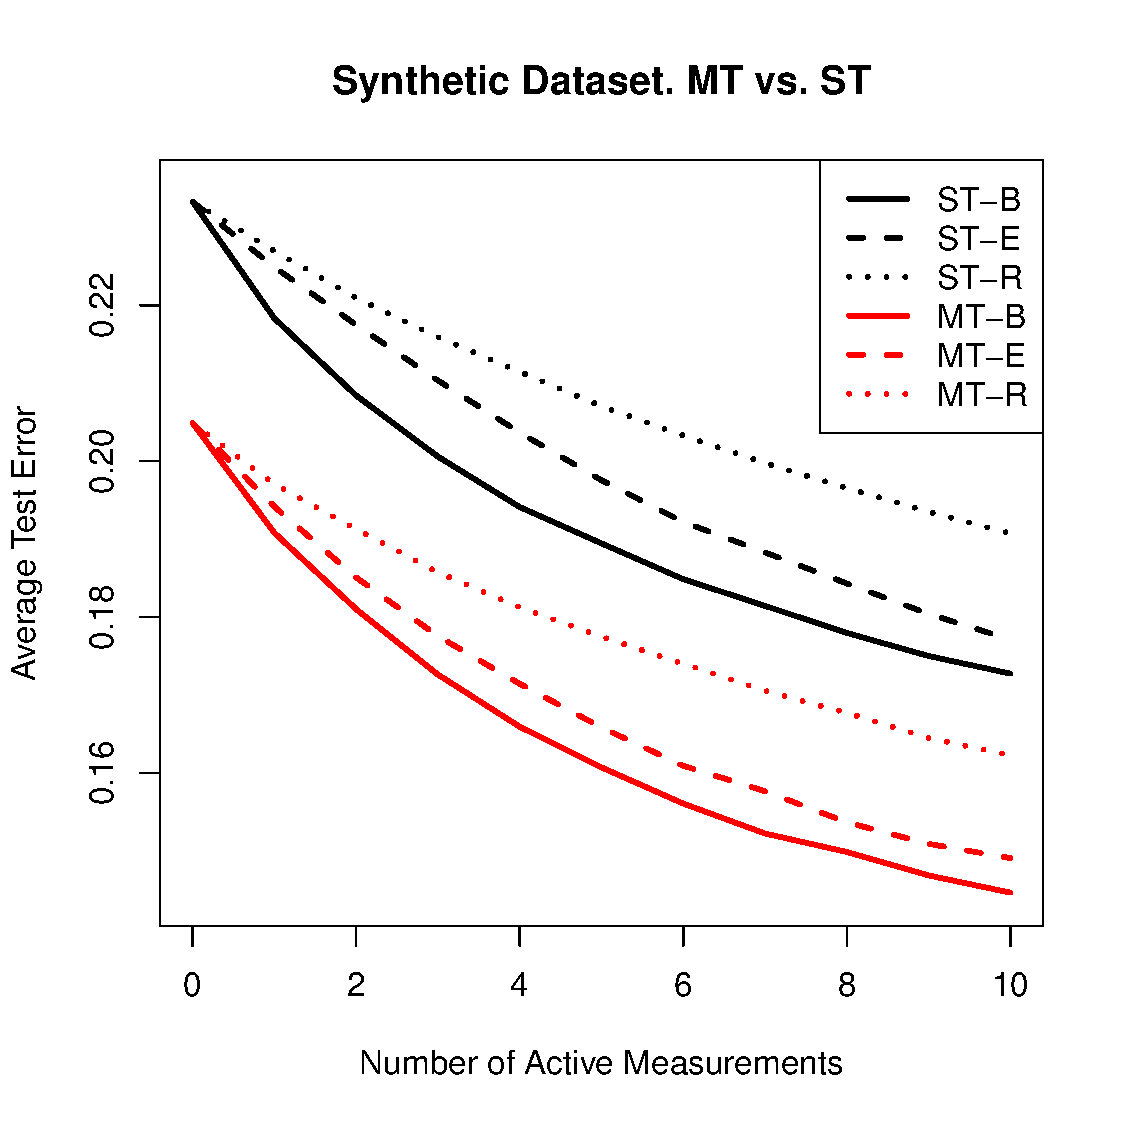
\includegraphics[scale = 0.36]{figs/plotsSyntheticData/plotSyntheticDatasetSTvsMT.pdf}
\hspace{0.5cm}
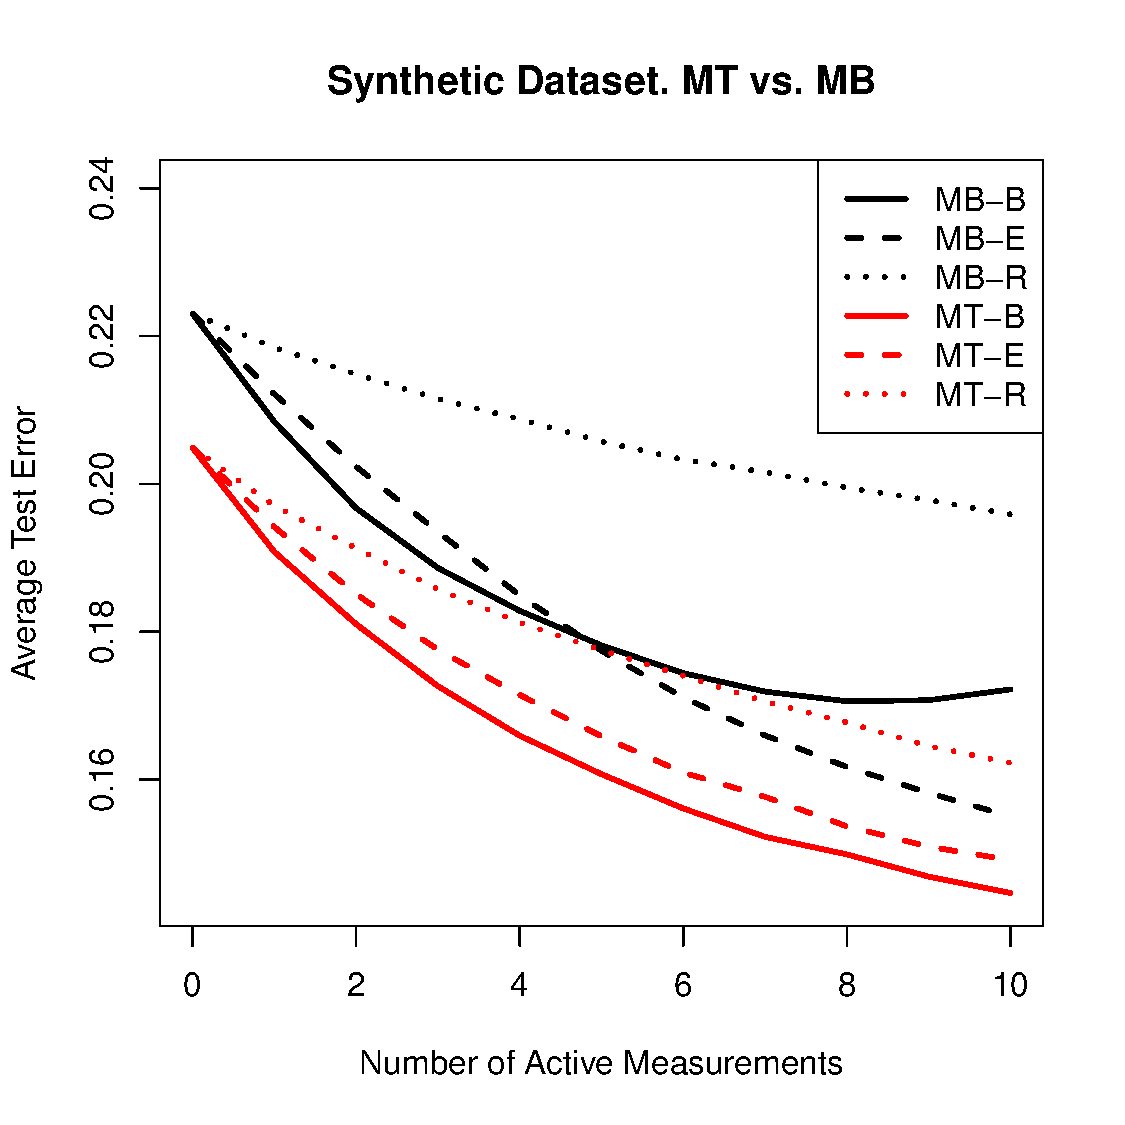
\includegraphics[scale = 0.36]{figs/plotsSyntheticData/plotSyntheticDatasetMBvsMT.pdf}\\
\vspace{0.5cm}
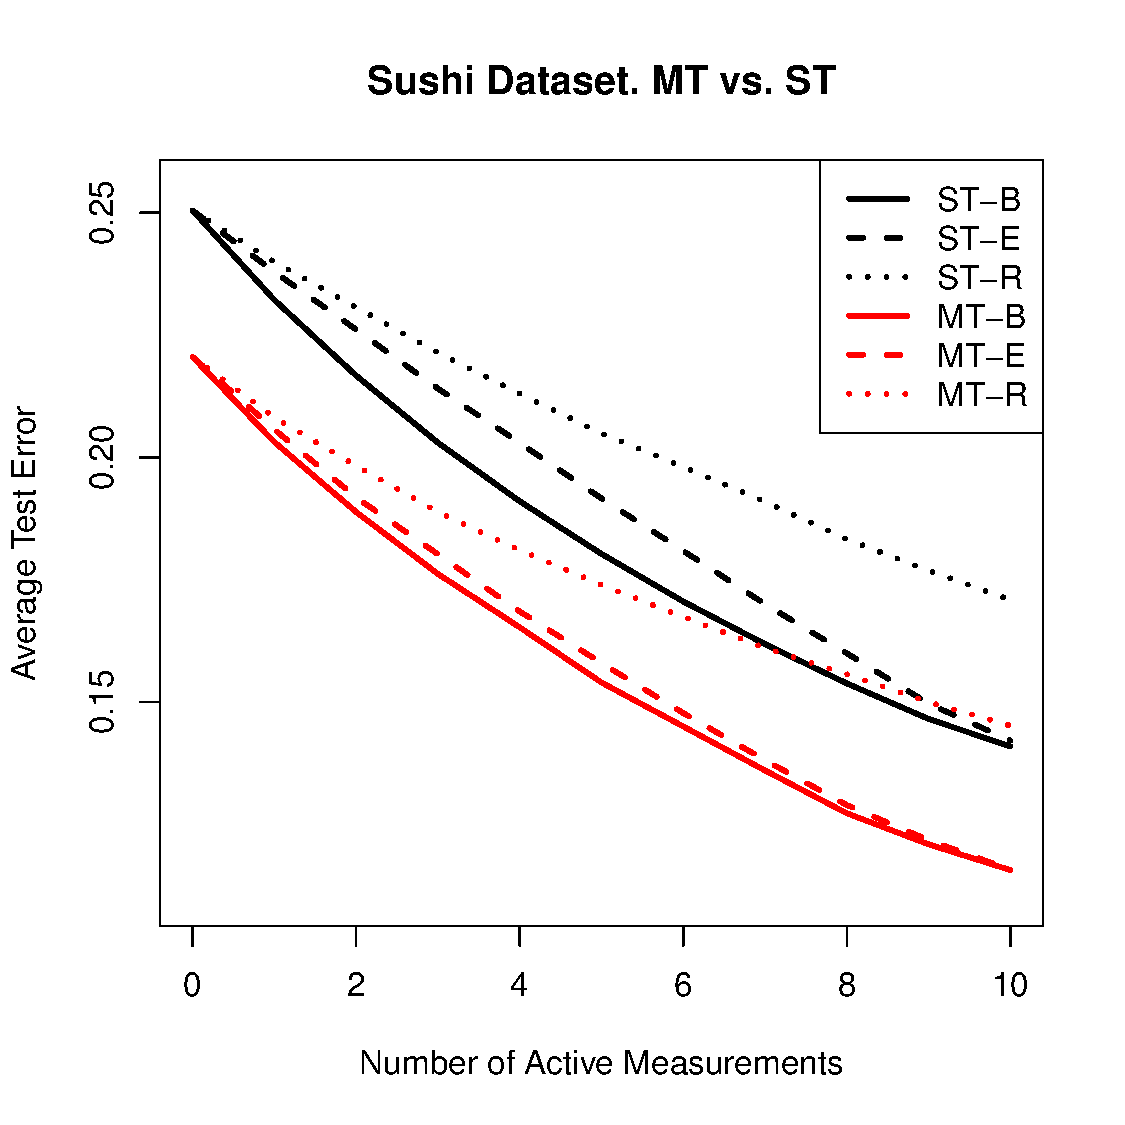
\includegraphics[scale = 0.36]{figs/plotsSushiData/plotSushiDatasetSTvsMT.pdf}
\hspace{0.5cm}
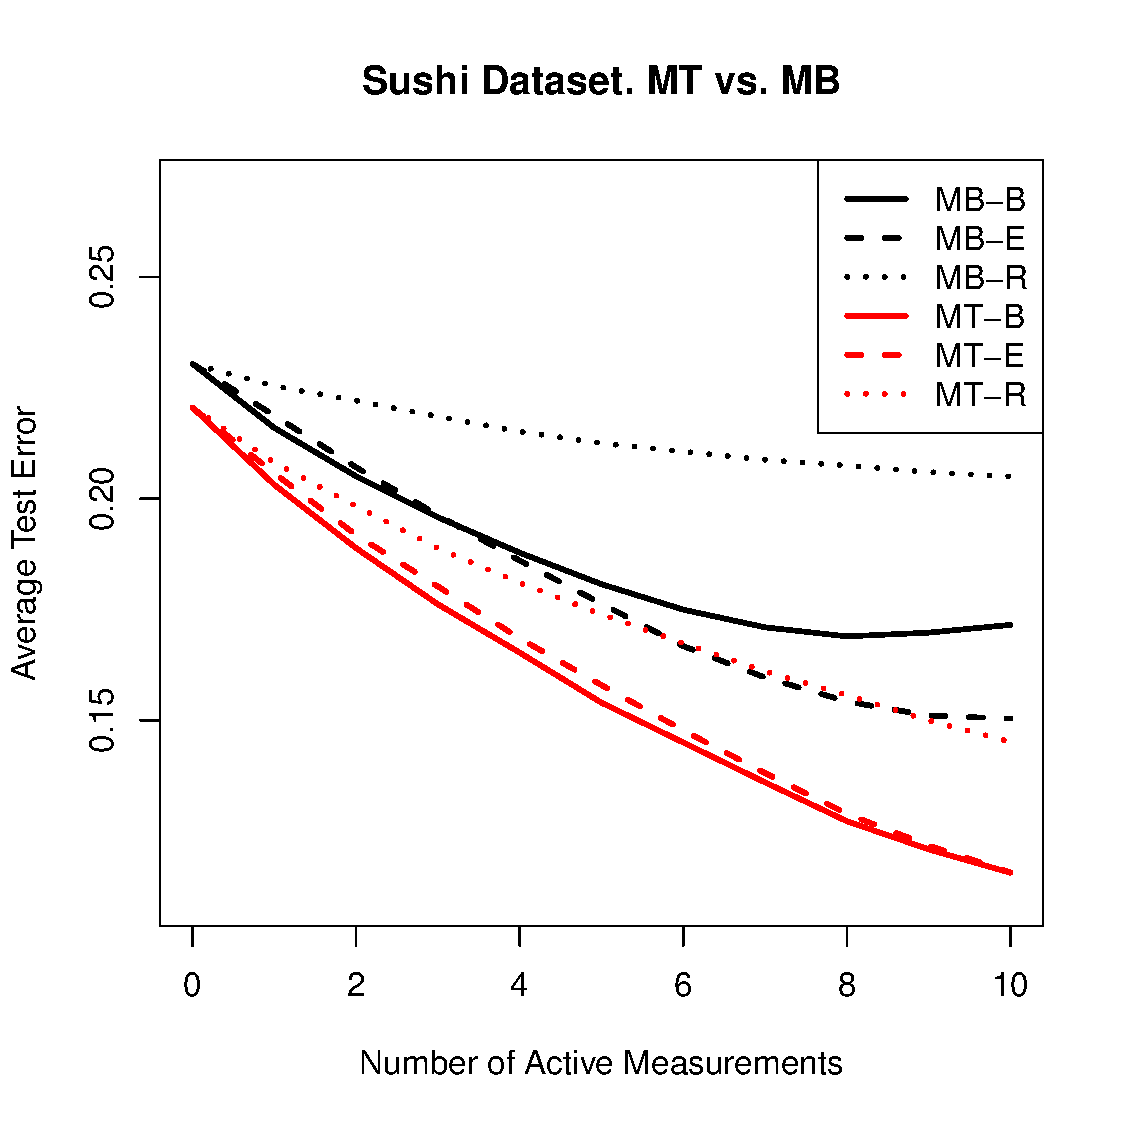
\includegraphics[scale = 0.36]{figs/plotsSushiData/plotSushiDatasetMBvsMT.pdf}
\caption{Top left, average test error as a function of the number of active measurements from the pool sets
for the proposed multi-task approach (MT) in the simulated data using BALD (MT-B), entropy (MT-E) and a random method (MT-R)
for the selection of the most informative points in the pool set. This plot also shows the average test error on the simulated data for
the single task method (ST) using BALD (ST-B), entropy (ST-E) and the random approach (ST-R). Top right,
comparison on the simulated data of MT-B, MT-E and MT-R with respect to the 
multi-task method given by \cite{Birlutiu2011} (MB) using BALD (MB-B), entropy (MB-E) and random (MB-R)
strategies for the selection of the most informative points.
Bottom left, comparison on the Sushi dataset of the results of MT-B, MT-E and MT-R with respect to ST-B, ST-E and ST-R.
Bottom right, comparison on the Sushi dataset of the results of MT-B, MT-E and MT-R with respect to MB-B, MB-E and MB-R.
}\label{fig:resultsSimulatedData}
\end{center}
\end{figure}

In the previous experiments with simulated data, MT obtained the best performance. This was expected because the data were actually sampled
from the probabilistic model assumed by this method. To obtain more representative results, we perform another series of experiments
with real-world data. In particular, we evaluate the performance of MT on the Sushi dataset \citep{kamishima2003}.
This dataset contains complete rankings given by 5000 users over a total of $I = 10$ different types of sushi,
where each sushi is represented by a set of features including style, major group, minor group, heaviness, consumption
frequency, normalized price and sell frequency. The first three featuers are categorical. We encoded these
features using dummy binary variables \citep{bonilla2010}. 
Each sushi is represented by a 15-dimensional feature vector. The protocol used in these experiments is
the same as before with two exceptions. First, we reduce the size of the dataset by
randomly sub-sampling $U=1000$ users. Second, for each of these users, the available preference data are 
now randomly split into training, pool and test sets with 10, 20 and 25 elements, respectively.
The configuration for the different methods is also the same as before.
However, we now use a total of $D=50$ latent functions in MT. 
The results obtained by this method are not very sensitive to the exact value of this parameter as long as it is not excessively low.
Finally, we always standardize the item features so that they have zero mean and unit standard deviation in the training set.
This procedure increases the probability that the value chosen for the length-scale parameter of the
preference kernel ($\sigma = 1$) leads to accurate results. 
In practice, the kernel parameter should be learned to obtain the best possible performance. 
This can be done in the proposed multi-task approach (MT) and in the single task method (ST) by searching for the parameter value that
maximizes the EP approximation of the model evidence. The cost of this search is too expensive for the proposed experimental protocol.
Nevertheless, we expect that using the same value for the kernel parameter in all methods leads to an unbiased comparison of performances.
The last part of this section contains experiments that indicate that the EP approximation of the model evidence can be used to successfully
select the kernel length-scale parameter in the proposed multi-task model.

The plot on the bottom left of Figure \ref{fig:resultsSimulatedData} shows the average test error of the proposed multi-task method,
MT-B, MT-E and MT-R, as a function of the number of active measurements obtained from
the pool set of each user in the experiments with the Sushi dataset.
The average test error of ST-B, ST-E and ST-R is also shown.
The MT techniques are markedly superior to the corresponding ST methods.
The differences between the BALD and entropy alternatives are also significant, with BALD outperforming entropy in general.
However, for more than 5 active measurements the errors of MT-B and ST-B seem to converge to the errors of MT-E and ST-E, respectively.
This result is likely to have its origin in the reduced size of the pool set which only contains 20 points in this case.
The bottom right plot in Figure \ref{fig:resultsSimulatedData} shows a comparison of the
average test errors of the MT and MB variants. In this case, the proposed multi-task technique with the BALD criterium (MT-B)
also obtains the best performance.
Table \ref{tab:resultsSimulated} shows the average test error and corresponding standard deviation for each method
on the Sushi dataset when a total of 0, 3, 5, 7 and 10 active measurements have been completed. The results of the
best performing method have been high-lighted in boldface.

\begin{table*} \centering
\caption{Results for the Sushi dataset: test error $\pm 1\,\mathrm{s.d}$. Best performing algorithms highlighted in bold face.}
\label{tab:resultsSushi}
\resizebox{\textwidth}{!}{
\begin{tabular}{c@{\hspace{0.2cm}}r@{$\pm$}l@{\hspace{0.2cm}}r@{$\pm$}l@{\hspace{0.2cm}}r@{$\pm$}l@{\hspace{0.2cm}}r@{$\pm$}l@{\hspace{0.2cm}}r@{$\pm$}l@{\hspace{0.2cm}}r@{$\pm$}l@{\hspace{0.2cm}}r@{$\pm$}l@{\hspace{0.2cm}}r@{$\pm$}l@{\hspace{0.2cm}}r@{$\pm$}l}
\hline
\bf{ $\bm n$}& \multicolumn{2}{c}{ \bf{ MT-B }}& \multicolumn{2}{c}{ \bf{ MT-E }}& \multicolumn{2}{c}{ \bf{ MT-R }}& \multicolumn{2}{c}{ \bf{ ST-B }}& \multicolumn{2}{c}{ \bf{ ST-E }}& \multicolumn{2}{c}{ \bf{ ST-R }}& \multicolumn{2}{c}{ \bf{ MB-B }}& \multicolumn{2}{c}{ \bf{ MB-E }}& \multicolumn{2}{c}{ \bf{ MB-R }}\\
\hline
0&\bf{22.05} & \bf{0.4}& \bf{22.05} & \bf{0.4} & \bf{22.05} & \bf{0.4} & 25.05 & 0.4& 25.05 & 0.4& 25.05 & 0.4& 23.04 & 0.5& 23.04 & 0.5& 23.04 & 0.5\\
3&\bf{17.62} & \bf{0.4}& 18.02 & 0.3& 18.88 & 0.3& 20.30 & 0.4& 21.41 & 0.4& 22.14 & 0.3& 19.58 & 0.5& 19.63 & 0.4& 21.85 & 0.5\\
5&\bf{15.40} & \bf{0.3}& 15.79 & 0.2& 17.39 & 0.3& 18.03 & 0.4& 19.16 & 0.3& 20.49 & 0.4& 18.07 & 0.4& 17.63 & 0.4& 21.25 & 0.5\\
7&\bf{13.60} & \bf{0.3}& 13.81 & 0.2& 16.11 & 0.4& 16.18 & 0.3& 17.00 & 0.3& 19.09 & 0.3& 17.10 & 0.4& 15.97 & 0.4& 20.87 & 0.5\\
10&\bf{11.56} & \bf{0.2}& \bf{11.57} & \bf{0.2} & 14.52 & 0.3& 14.09 & 0.3& 14.21 & 0.3& 17.09 & 0.3& 17.15 & 0.4& 15.04 & 0.3& 20.50 & 0.4\\

\hline
\end{tabular}
}
\end{table*}


Finally, we perform an additional experiment to show
that the approximation of the evidence given by EP (\ref{eq:EPevidenceApprox}) can be used to select
the kernel length-scale parameter $\sigma$. We use the same simulated data that was described at the begining of this section.
For each of the 25 initial training sets with $500 \times 10$ observations (10 observations per user),
we evaluate the value of $\log \mathcal{P}(\mathbf{T}^{(\mathcal{D})}|\mathbf{X},\ell)$, as estimated by EP,
for different values of $\log \sigma$. Ideally, we would like the average evidence given by EP
to peak at the value of $\sigma$ that was used to generate the data, that is, $\sigma = 1$.
Figure \ref{fig:evidencePlot} shows that this is the case.

\begin{figure}
\begin{center}
\includegraphics[scale = 0.36]{figs/evidencePlots/evidence.pdf}
\caption{
Average value of $\log \mathcal{P}(\mathbf{T}^{(\mathcal{D})}, \mathbf{X}, \ell)$ as estimated by EP with respect to $\log \sigma$. 
The red arrows indicate the size of the empirical standard deivation in the EP estimates for the evidence.
The evidence has its maximum at $\sigma = 1$, the value used to generate the data.
}\label{fig:evidencePlot}
\end{center}
\end{figure}
